\newpage
\subsection{Μελέτη των N-bit Predictors}
\vspace{3mm}

\subsubsection{Μελέτη για σταθερό αριθμό BHT Entries}
Στο σημείο αυτό μελετάται η απόδοση των N-bit Predictors για διαφορετικές τιμές
του N = 1, 2, 3, 4, ενώ τα entries διατηρούνται σταθερά και ίσα με 16Κ.Τα N-bit
υλοποιούν ένα saturating up-down counter. Επιπλέον, υλοποιείται ένας predictor
με το κάτωθι FSM:

\begin{center}
   \vspace{3mm}
      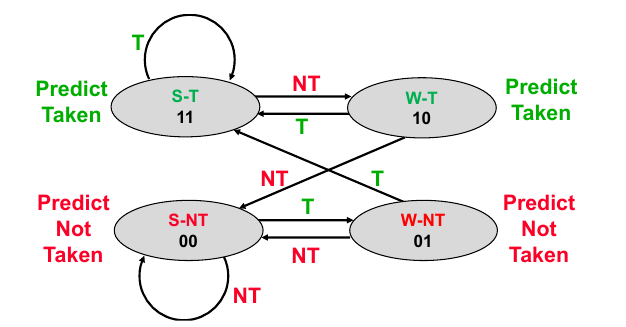
\includegraphics[width=0.65\textwidth, frame]{./imgs/fsm.png}
   \vspace{6mm}
\end{center}


\vspace{1em}    
Η σύγκριση των predictors γίνεται με βάση τα direction Mispredictions Per
Thousand Instructions (direction MPKI). Ακολουθούν τα διαγράμματα που
προέκυψαν και ο σχετικός σχολιασμός τους:

   \begin{minipage}{\textwidth}
      \begin{center}
         \fbox{\textlatin{\textbf{\textit{403-gcc}}}}\\
         \vspace{3mm}
         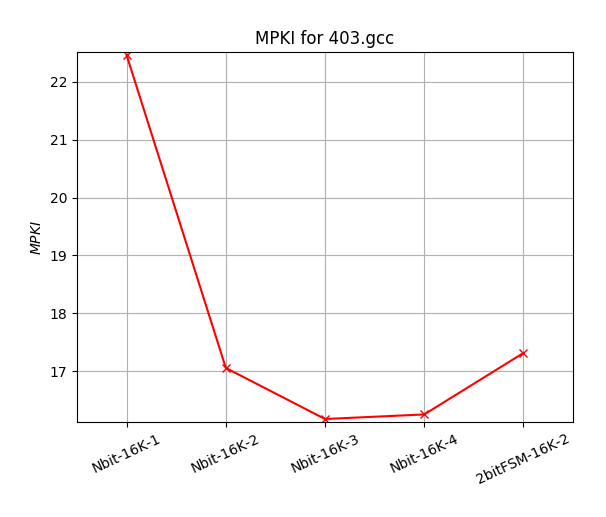
\includegraphics[width=0.65\textwidth, frame]{./graphs/4-2i/403-gcc.png}
         \vspace{6mm}
      \end{center}
   \end{minipage}

   \begin{minipage}{\textwidth}
      \begin{center}
         \fbox{\textlatin{\textbf{\textit{429-mcf}}}}\\
         \vspace{3mm}
         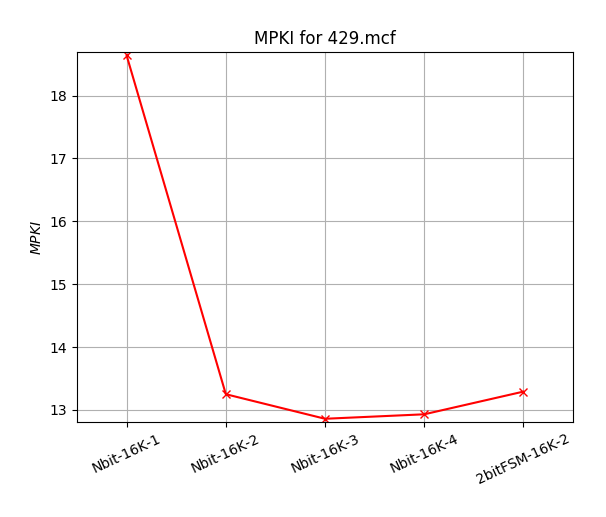
\includegraphics[width=0.65\textwidth, frame]{./graphs/4-2i/429-mcf.png}
         \vspace{6mm}
      \end{center}
   \end{minipage}

   \begin{minipage}{\textwidth}
      \begin{center}
         \fbox{\textlatin{\textbf{\textit{434-zeusmp}}}}\\
         \vspace{3mm}
         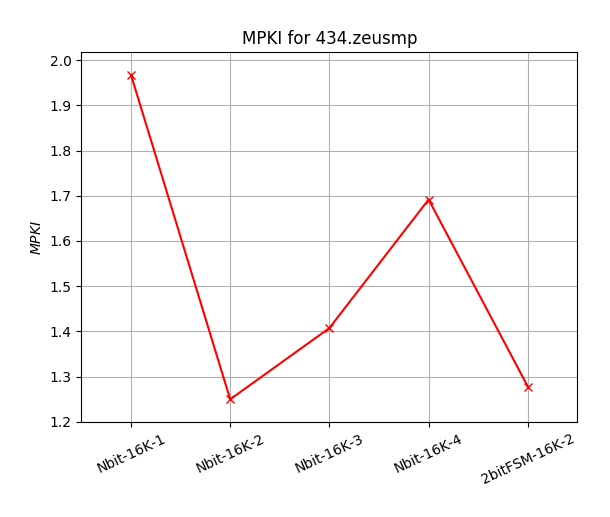
\includegraphics[width=0.65\textwidth, frame]{./graphs/4-2i/434-zeusmp.png}
         \vspace{6mm}
      \end{center}
   \end{minipage}

   \begin{minipage}{\textwidth}
      \begin{center}
         \fbox{\textlatin{\textbf{\textit{436-cactusADM}}}}\\
         \vspace{3mm}
         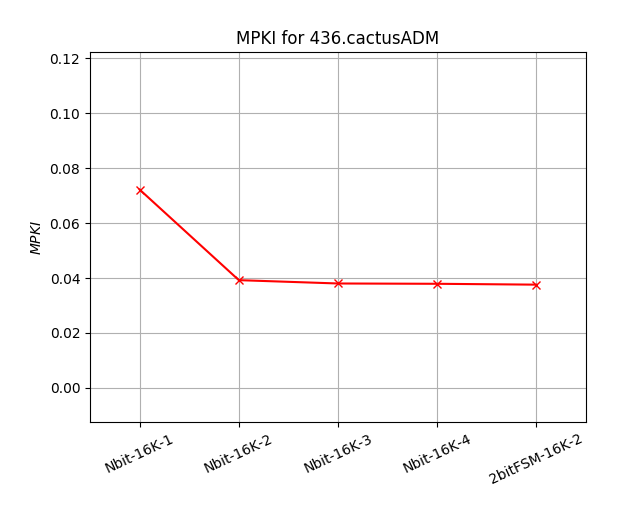
\includegraphics[width=0.65\textwidth, frame]{./graphs/4-2i/436-cactusADM.png}
         \vspace{6mm}
      \end{center}
   \end{minipage}

   \begin{minipage}{\textwidth}
      \begin{center}
         \fbox{\textlatin{\textbf{\textit{445-gobmk}}}}\\
         \vspace{3mm}
         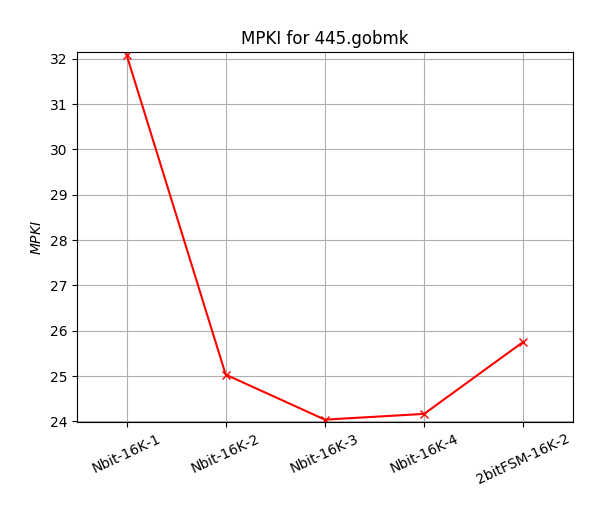
\includegraphics[width=0.65\textwidth, frame]{./graphs/4-2i/445-gobmk.png}
         \vspace{6mm}
      \end{center}
   \end{minipage}

   \begin{minipage}{\textwidth}
      \begin{center}
         \fbox{\textlatin{\textbf{\textit{450-soplex}}}}\\
         \vspace{3mm}
         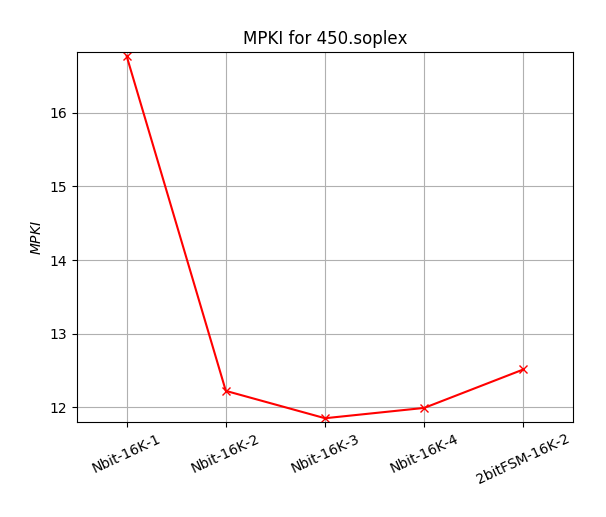
\includegraphics[width=0.65\textwidth, frame]{./graphs/4-2i/450-soplex.png}
         \vspace{6mm}
      \end{center}
   \end{minipage}

   \begin{minipage}{\textwidth}
      \begin{center}
         \fbox{\textlatin{\textbf{\textit{456-hmmer}}}}\\
         \vspace{3mm}
         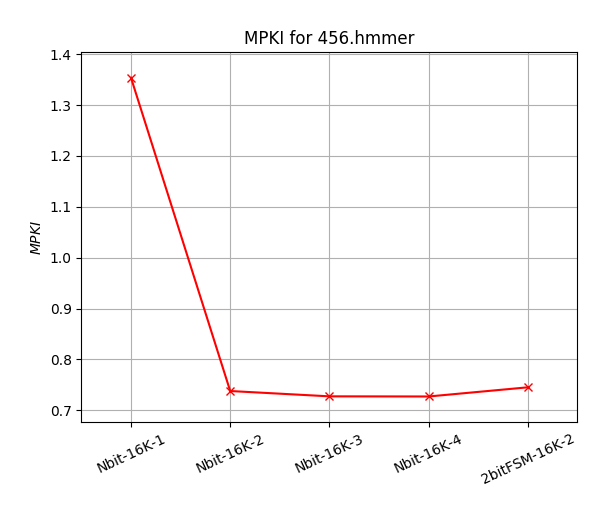
\includegraphics[width=0.65\textwidth, frame]{./graphs/4-2i/456-hmmer.png}
         \vspace{6mm}
      \end{center}
   \end{minipage}

   \begin{minipage}{\textwidth}
      \begin{center}
         \fbox{\textlatin{\textbf{\textit{458-sjeng}}}}\\
         \vspace{3mm}
         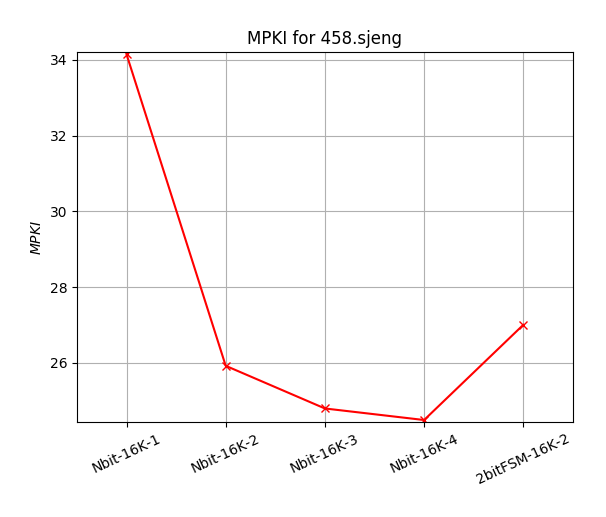
\includegraphics[width=0.65\textwidth, frame]{./graphs/4-2i/458-sjeng.png}
         \vspace{6mm}
      \end{center}
   \end{minipage}

   \begin{minipage}{\textwidth}
      \begin{center}
         \fbox{\textlatin{\textbf{\textit{459-GemsFDTD}}}}\\
         \vspace{3mm}
         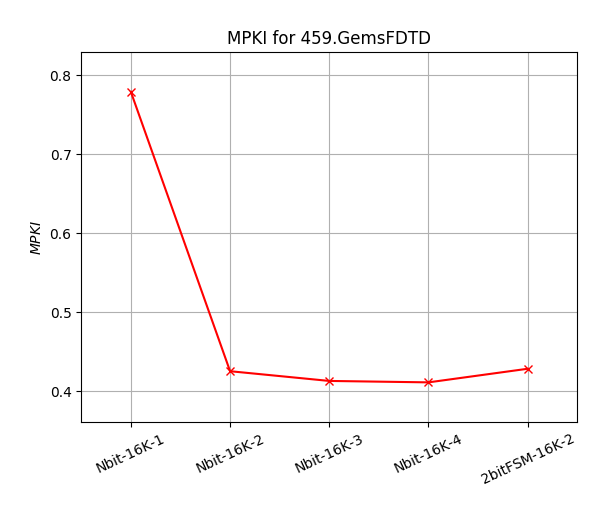
\includegraphics[width=0.65\textwidth, frame]{./graphs/4-2i/459-GemsFDTD.png}
         \vspace{6mm}
      \end{center}
   \end{minipage}

   \begin{minipage}{\textwidth}
      \begin{center}
         \fbox{\textlatin{\textbf{\textit{471-omnetpp}}}}\\
         \vspace{3mm}
         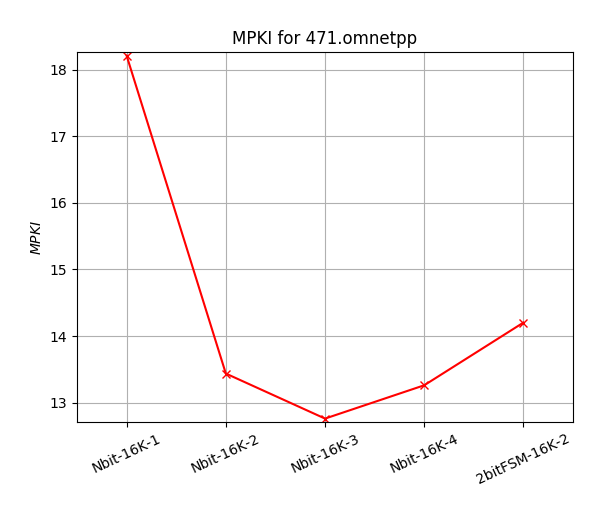
\includegraphics[width=0.65\textwidth, frame]{./graphs/4-2i/471-omnetpp.png}
         \vspace{6mm}
      \end{center}
   \end{minipage}

   \begin{minipage}{\textwidth}
      \begin{center}
         \fbox{\textlatin{\textbf{\textit{473-astar}}}}\\
         \vspace{3mm}
         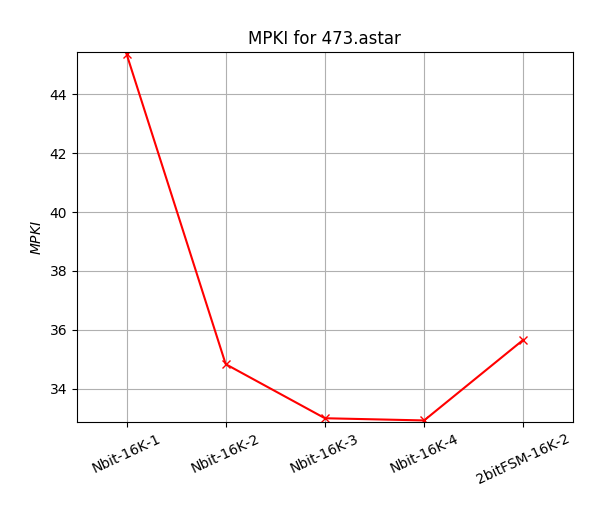
\includegraphics[width=0.65\textwidth, frame]{./graphs/4-2i/473-astar.png}
         \vspace{6mm}
      \end{center}
   \end{minipage}

   \begin{minipage}{\textwidth}
      \begin{center}
         \fbox{\textlatin{\textbf{\textit{483-xalancbmk}}}}\\
         \vspace{3mm}
         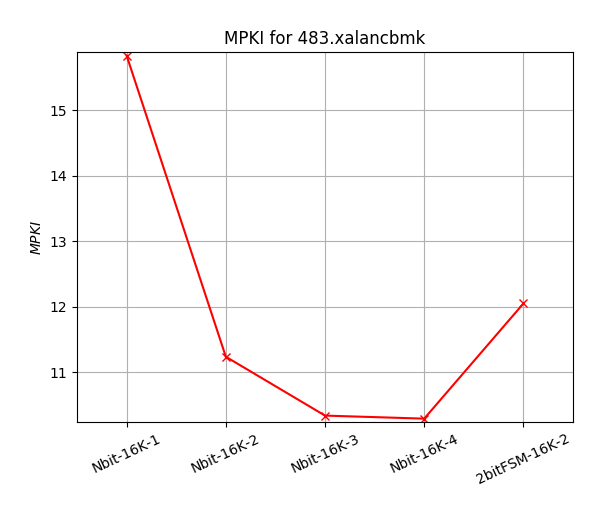
\includegraphics[width=0.65\textwidth, frame]{./graphs/4-2i/483-xalancbmk.png}
         \vspace{6mm}
      \end{center}
   \end{minipage}

   \begin{minipage}{\textwidth}
      \begin{center}
         \fbox{\textlatin{\textbf{\textit{Geometric Average}}}}\\
         \vspace{3mm}
         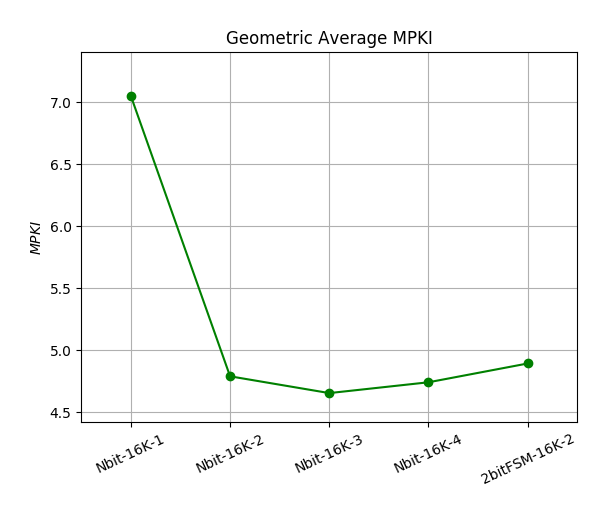
\includegraphics[width=0.65\textwidth, frame]{./graphs/4-2i/mean.png}
         \vspace{6mm}
      \end{center}
   \end{minipage}

\paragraph{Συμπεράσματα-Σχόλια}
    Από της μορφές των καμπυλών στα παραπάνω διαγράμματα παρατηρούμε πως 11 στα
    12 benchmarks παρουσιάζουν βελτίωση καθώς το πλήθος των bits του predictor
    αυξάνει, δηλάδή η μετρική dMPKI φθίνει καθώς τα bits αυξάνονται. Η μόνη
    διαφορετική ως προς την μορφή καμπύλη αντιστοιχεί στο μετρόπρόγραμμα
    434.zeusmp για το οποίο το μικρότερο MPKI αντιστοιχεί σε 2-bit predictor.
    Ωστόσο πρέπει να επισημάνουμε πως για το εν λόγω μετροπρόγραμμα η μεταβολή
    το MPKI είναι ήδη αρκετά χαμηλό και η μεταβολή του με τη χρήση διαφορετικών
    Nbit-Predictors είναι αρκετά μικρή (εύρος 1.2 εώς 2.0 Misses Per
    KILOInstructions), άρα δεν μας επηρεάζει και πολύ.

    Βοηθάει να αποκτήσουμε μία σαφώς πιο συνολική εικόνα και το διάγραμμα
    γεωμετρικών μέσων των παραπάνω τιμών, όπου εκεί επιβεβαιώνουμε τα
    προηγούμενα συμπεράσματα. Επιπλέον, να σημειώσουμε ότι το FSM που
    υλοποιήσαμε αποδίδει καλύτερα μονάχα σε σχέση με τον 1bit Predictor. Σαφώς η
    \textbf{καλύτερη επιλογή φαίνεται να είναι ο 4-bit Predictor}.

